%!LW recipe=latexmk (latexmkrc)

\documentclass[10pt,aspectratio=169,notheorems]{beamer}

\usetheme[palette = frappe]{slidemint}
\slidemintsetup{
    footer-left = {\textcopyright~Michael Tiemann, 2026}
}

\usepackage{macromint}
\usepackage{figmint}
\usepackage{booktabs}
\usepackage{array}

\title{HPC in Europe}
\subtitle{Through an Academic's Lens}
\author{Dr.~Michael Tiemann}
\institute{Project Minerva\\T\"ubingen AI Center\\University of T\"ubingen}
\date{May 20, 2026}

\newcommand*{\EUR}[1]{\mbox{€\,#1}}

\begin{document}

\begin{frame}[plain]
    \begin{tikzpicture}[remember picture,overlay]
        \ifSlidemintDarkMode
            \node[anchor=west,xshift=-3mm] at (current page.west) {
                
\includegraphics[height=\paperheight,keepaspectratio]{graphics/title-graphic-light.pdf}
            };
            \node[anchor=north east,yshift=-3mm,xshift=-5mm] at (current page.north east) {
                
\includegraphics[width=2.5cm]{graphics/affiliation-logo-light.pdf}
            };
            % Collaboration logo (Uni + MPI) removed — uncomment to re-add or replace.
            % \node[anchor=south east,yshift=3mm,xshift=-3mm] at (current page.south east) {
            %     
\includegraphics[width=8cm]{graphics/collaboration-logo-light.pdf}
            % };
            \node[anchor=south,yshift=3mm] at (current page.south) {
                \scriptsize\textcolor{SlidemintMuted}{Original talk: B\'alint Mucs\'anyi \,\textbar\, \href{https://github.com/bmucsanyi/hpc_talk}{github.com/bmucsanyi/hpc\_talk}}
            };
            \node[anchor=south east,yshift=3mm,xshift=-1cm] at (current page.south east) {
                
\includegraphics[height=1cm]{graphics/eu-cofunded.jpg}
                \hspace{.6em}
                
\includegraphics[height=1cm]{graphics/minerva-logo.png}
            };
        \else
            \node[anchor=west,xshift=-3mm] at (current page.west) {
                
\includegraphics[height=\paperheight,keepaspectratio]{graphics/title-graphic-color.pdf}
            };
            \node[anchor=north east,yshift=-3mm,xshift=-5mm] at (current page.north east) {
                
\includegraphics[width=2.5cm]{graphics/affiliation-logo-color.pdf}
            };
            % Collaboration logo (Uni + MPI) removed — uncomment to re-add or replace.
            % \node[anchor=south east,yshift=3mm,xshift=-3mm] at (current page.south east) {
            %     
\includegraphics[width=8cm]{graphics/collaboration-logo-color.pdf}
            % };
            \node[anchor=south,yshift=3mm] at (current page.south) {
                \scriptsize\textcolor{SlidemintMuted}{Original talk: B\'alint Mucs\'anyi \,\textbar\, \href{https://github.com/bmucsanyi/hpc_talk}{github.com/bmucsanyi/hpc\_talk}}
            };
            \node[anchor=south east,yshift=3mm,xshift=-1cm] at (current page.south east) {
                
\includegraphics[height=1cm]{graphics/eu-cofunded.jpg}
                \hspace{.6em}
                
\includegraphics[height=1cm]{graphics/minerva-logo.png}
            };
        \fi
        \node[anchor=center,xshift=.1\paperwidth] at (current page.center) {
            \begin{minipage}[c][\dimexpr\paperheight-0.1062\paperwidth-2em\relax][c]{\textwidth}
                \centering
                {\usebeamerfont{title}\usebeamercolor[fg]{title}\inserttitle\par}
                \vskip0.25em
                {\usebeamerfont{subtitle}\usebeamercolor[fg]{subtitle}\insertsubtitle\par}
                \vskip.5em
                {\usebeamerfont{author}\usebeamercolor[fg]{author}\insertauthor\par}
                \vskip.5em
                {\usebeamerfont{institute}\usebeamercolor[fg]{institute}\insertinstitute\par}
                \vskip.3em
                {\usebeamerfont{date}\usebeamercolor[fg]{date}\insertdate\par}
                \vfill
            \end{minipage}
        };
    \end{tikzpicture}
\end{frame}

\begin{frame}
    \frametitle{The GPU need of an ML/CV PhD}
    \framesubtitle{Not a niche problem}
    \begin{itemize}
        \item Modern research runs on \SlidemintTextbf{training runs}: large models, large datasets, several seeds.
        \item A competitive study needs \SlidemintTextbf{hundreds of GPU-days}; ablations, hyperparameter search, and baselines \SlidemintEmph{multiply} that again.
        \item A local desktop with 1--2 GPUs is fine for \SlidemintEmph{prototyping}, not for the campaign---if you're lucky and you have one and it satisfies your needs.
        \item Buying the hardware yourself is not an option---so researchers climb a ladder of \SlidemintTextbf{shared resources}.
    \end{itemize}

    \vspace{2em}
    \textcolor{SlidemintMuted}{One GPU already costs a small fortune: the price tag is the next section.}
\end{frame}

% ----------------------------------------------------------------------
% Original first slide of B\'alint Mucs\'anyi's talk, restored verbatim.
% Kept here as an ADDITIONAL slide: the deck no longer opens with it, but
% removing it was not intended. Comment out the frame to drop it again.
% ----------------------------------------------------------------------
\begin{frame}
    \frametitle{An example project}
    \framesubtitle{A project from T\"ubingen's B\'alint Mucs\'anyi}
    \begin{itemize}
        \item Needed \SlidemintTextbf{2--5 H100 GPU-years} for two projects.
        \item T\"ubingen's local AI cluster, two machines named Galvani and Ferranti, throttled the concurrent-job count.
        \item And thus he set out on a quest for compute.
    \end{itemize}
\end{frame}

\begin{frame}
    \frametitle{From one desktop GPU to EuroHPC}
    \framesubtitle{The compute ladder}
    \begin{center}
    \begin{tabular}{@{}>{\bfseries\color{SlidemintStrong}}r@{\;}c@{\quad}l@{}}
        Desktop        &       & 1--2 GPUs, always yours; prototyping and debugging \\
                       & $\downarrow$ & \\
        University     &       & group cluster / group quota; e.g.\ the ML Cloud \\
                       & $\downarrow$ & \\
        State          &       & Helix (Baden-W\"urttemberg) \\
                       & $\downarrow$ & \\
        Federal        &       & NHR (national Tier-2), GCS (national Tier-1) \\
                       & $\downarrow$ & \\
        \SlidemintTextbf{EuroHPC JU} & & the European fleet: MareNostrum 5, LUMI, Leonardo, JUPITER \\
    \end{tabular}
    \end{center}

    \vspace{2em}
    \textcolor{SlidemintMuted}{Each rung up buys scale --- and costs latency. Proposal time is part of throughput.}
\end{frame}



% \begin{frame}
%     \frametitle{What this talk is}
%     \framesubtitle{And what it is not}
%     \SlidemintTextbf{Not} HPC 101: most of you have already used a cluster.

%     \vspace{0.5em}
%     What we'll be centered around: \SlidemintEmph{throughput is not \texttt{sinfo}}.
%     $$\text{throughput} \approx \text{GPUs} \times \text{reliability} \times \text{queue} \times \text{proposal latency} \times \text{communication} \times \text{best practices}$$

%     \vspace{0.5em}
%     We climb the \SlidemintTextbf{GPU ladder}: \SlidemintTextbf{desktop} $\to$ \SlidemintTextbf{university} $\to$ \SlidemintTextbf{state} $\to$ \SlidemintTextbf{federal} $\to$ \SlidemintTextbf{Europe}.

%     \vspace{0.5 em}
%     Then: how to make the most out of the resources.
% \end{frame}

\section{The cost of compute}

\begin{frame}
    \frametitle{HPC is super expensive!}
    \framesubtitle{A100 40 GB}
    \begin{center}
    \begin{tabular}{@{}l@{\hspace{0.75em}}r@{}}
        \toprule
        Buy new in 2020              & \textcolor{SlidemintMuted}{$\sim$\,\EUR{9{,}000}} \\
        Buy second-hand today        & \SlidemintTextbf{\EUR{4{,}500}--\EUR{6{,}500}} \\
        Power for a GPU-year (250\,W, \EUR{0.30}/kWh) & \EUR{657} \\
        Rent on Lambda Labs (\$1.29/h) & \EUR{10{,}400} \\
        Rent on Google Cloud (\$3.67/h)    & \SlidemintTextbf{\EUR{29{,}600}} \\
        \bottomrule
    \end{tabular}
    \end{center}
\end{frame}

\begin{frame}
    \frametitle{HPC is super expensive!}
    \framesubtitle{H100 80 GB}
    \begin{center}
    \begin{tabular}{@{}l r@{}}
        \toprule
        Buy new in 2022              & \textcolor{SlidemintMuted}{$\sim$\,\EUR{30{,}000}} \\
        Buy new today                & \SlidemintTextbf{\EUR{25{,}000}--\EUR{35{,}000}} \\
        Power for a GPU-year (700\,W, \EUR{0.30}/kWh) & \EUR{1{,}840} \\
        Rent on RunPod (\$3.29/h SXM)  & \EUR{26{,}500} \\
        Rent on Google Cloud (\$11/h)      & \SlidemintTextbf{\EUR{88{,}700}} \\
        \bottomrule
    \end{tabular}
    \end{center}

    \vspace{2em}
    \textcolor{SlidemintMuted}{H100 power draw is $\sim 2.8\times$ A100.\\Google Cloud H100 is $\sim 3\times$ Google Cloud A100.}
\end{frame}

\begin{frame}
    \frametitle{B\'alint's project, priced four ways}
    \framesubtitle{2--5 H100 GPU-years, 64 H100s peak}
    \begin{center}
    \begin{tabular}{@{}l r@{}}
        \toprule
        Buy the 64 cards outright              & \SlidemintTextbf{\EUR{1.8}M--\EUR{2.5}M} \\
        Power the cards for 2--5 GPU-years     & \EUR{3{,}700}--\EUR{9{,}200} \\
        Rent on a budget cloud (RunPod-tier)   & \EUR{53{,}000}--\EUR{133{,}000} \\
        Rent on Google Cloud                    & \SlidemintTextbf{\EUR{177{,}000}--\EUR{443{,}000}} \\
        \bottomrule
    \end{tabular}
    \end{center}

    \vspace{2em}
    \textcolor{SlidemintMuted}{The reason European HPC exists in this form is that \SlidemintEmph{nobody in academia} pays the right column.}
\end{frame}

\begin{frame}
    \frametitle{Why a deep-learning researcher ever needs this}
    \framesubtitle{Parameter spaces are huge}
    My work: \SlidemintTextbf{optimization}, \SlidemintTextbf{model editing}, \SlidemintTextbf{unlearning}: all of them live in \SlidemintEmph{parameter space}.

    \vspace{0.5em}
    Working in parameter space means representing things like:
    \begin{itemize}
        \item gradients (1 copy of the model)
        \item Fisher / Hessian (formally: $d \times d$, with $d$ in the millions to billions)
        \item rank-$k$ subspaces from generalized eigenproblems
    \end{itemize}

    \vspace{2em}
    \textcolor{SlidemintMuted}{Each ``copy of the model'' is a unit of VRAM and they quickly add up.}
\end{frame}

\begin{frame}
    \frametitle{The parameter-space wall}
    \framesubtitle{One small model, one not-so-large LLM}
    \begin{columns}[t]
        \begin{column}{0.49\textwidth}
        \SlidemintTextbf{ResNet-50} \citep{he2016resnet}
        \begin{itemize}
            \item one fp32 copy: $\sim$100\,MB
            \item full Hessian: $\sim$2.6\,PB
            \item rank-1000 Fisher approximation: $\sim$\SlidemintTextbf{100\,GB}
        \end{itemize}
        \end{column}

        \begin{column}{0.49\textwidth}
        \SlidemintTextbf{Gemma 2 2B} \citep{gemmateam2024gemma2}
        \begin{itemize}
            \item one fp16 copy: $\sim$5\,GB
            \item rank-64 dense subspace: $\sim$\SlidemintTextbf{320\,GB}
            \item plus fp16 numerical instability
        \end{itemize}
        \end{column}
    \end{columns}

    \vspace{2em}
    \textcolor{SlidemintMuted}{The ``scalable'' solution is also expensive.}
\end{frame}

\begin{frame}
    \frametitle{H100 is not ``A100 + more VRAM''}
    \framesubtitle{Memory, bandwidth, and compute across GPU generations}
    \begin{columns}[t]
        \begin{column}{0.49\textwidth}
        \centering
        \figmintset{figure width=\linewidth, figure height=0.72\linewidth}
        \begin{figmintfigure}
            \begin{axis}[
                xlabel={Memory (GB)},
                ylabel={Bandwidth (TB/s)},
                xmin=0, xmax=180,
                ymin=0, ymax=5.6,
                xtick={32,80,141},
                ytick={1,2,3,4,5},
                nodes near coords align={anchor=west},
                every node near coord/.append style={xshift=4pt},
            ]
                \addplot+[figmint scatter, mark size=3pt, point meta=explicit symbolic, nodes near coords=\pgfplotspointmeta]
                    coordinates {
                        (32, 0.90)  [V100 32GB]
                        (40, 1.555) [A100 40GB]
                        (80, 2.039) [A100 80GB]
                        (80, 3.35)  [H100 80GB]
                        (141, 4.80) [H200 141GB]
                    };
            \end{axis}
        \end{figmintfigure}
        \end{column}

        \begin{column}{0.49\textwidth}
        \centering
        \figmintset{figure width=\linewidth, figure height=0.72\linewidth}
        \begin{figmintfigure}
            \begin{axis}[
                ylabel={FP16 Tensor TFLOPS},
                xtick={0,1,2,3,4},
                xticklabels={V100, A100-40, A100-80, H100, H200},
                xticklabel style={rotate=30, anchor=east},
                ymin=0, ymax=1150,
                ytick={0,200,400,600,800,1000},
                bar width=0.36cm,
                enlarge x limits=0.12,
                nodes near coords,
            ]
                \addplot+[figmint bar] coordinates {
                    (0, 125)
                    (1, 312)
                    (2, 312)
                    (3, 989)
                    (4, 989)
                };
            \end{axis}
        \end{figmintfigure}
        \end{column}
    \end{columns}

\end{frame}

\begin{frame}
    \frametitle{What each generation actually buys you}
    {
    \renewcommand{\arraystretch}{1.22}
    \begin{tabular}{@{}>{\bfseries\color{SlidemintStrong}}l@{\quad}p{0.82\textwidth}@{}}
        V100 & 16/32\,GB HBM2, $\sim$0.9\,TB/s. \newline First-gen tensor cores; no modern low-precision. \\
        A100 & Modern academic baseline. HBM2, 1.55--2.04\,TB/s, TF32 and BF16. \newline Many models run faster without you touching them. \\
        H100 & HBM3 at 3.35\,TB/s, 4th-gen tensor cores, FP8, Transformer Engine. \newline NVIDIA's own benchmarks: $\sim$3$\times$ BF16 GEMM, $\sim$5$\times$ FP8 GEMM vs A100. \\
        H200 & Same Hopper compute as H100. \newline \SlidemintTextbf{+76\,\% memory}, \SlidemintTextbf{+43\,\% bandwidth}. \newline A gift for memory-intensive workload. \\
        MI250X & EuroHPC's most-used accelerator (LUMI-G). \newline \SlidemintTextbf{ROCm}, not CUDA. \newline Not a drop-in for CUDA-optimized code.
    \end{tabular}
    }
\end{frame}

\section{HPC in T\"ubingen}

\begin{frame}
    \frametitle{ML Cloud on paper}
    \begin{columns}[t]
        \begin{column}{0.49\textwidth}
        \SlidemintTextbf{Galvani} (A100s, SLURM)
        \begin{itemize}
            \item 281 A100s
            \item $22 \times 8$, $11 \times 9$, $2 \times 3$ nodes
        \end{itemize}
        \end{column}

        \begin{column}{0.49\textwidth}
        \SlidemintTextbf{Ferranti} (H100s, SLURM)
        \begin{itemize}
            \item 120 H100s in $15 \times 8$ nodes
            \item 5 nodes: 192 CPUs, 2.06\,TB RAM
            \item 10 nodes: 384 CPUs, 2.32\,TB RAM
            \item Very strong NDR400 InfiniBand fabric
        \end{itemize}
        \end{column}
    \end{columns}
    \vspace{2em}
    \textcolor{SlidemintMuted}{Sounds like a lot. More than enough. Until things stop working.}
\end{frame}

\begin{frame}
    \frametitle{ML Cloud in practice}
    \begin{itemize}
        \item \SlidemintTextbf{Galvani:} 36 concurrent jobs, 36 GPUs.
        \item \SlidemintTextbf{Ferranti:} 8 concurrent jobs, no GPU cap. So in principle: 8 nodes $=$ \SlidemintTextbf{64 H100}.
        \item Caps are \SlidemintEmph{undocumented} and \SlidemintEmph{ad-hoc}; they can move again at any time.
    \end{itemize}

    \vspace{2em}
    \textcolor{SlidemintMuted}{Bulk requests make scheduling less efficient. 8 nodes for 3 days takes about a day of queue.}
\end{frame}

\begin{frame}[fragile]
    \frametitle{Compute is not to be taken for granted}
    \framesubtitle{A six-week ML Cloud weather report}
    {
    \footnotesize
    \begin{tabular}{@{}r l@{}}
        \textcolor{SlidemintMuted}{07 Apr} & Galvani: DNS issues \\
        \textcolor{SlidemintMuted}{08 Apr} & Galvani: scheduled maintenance starts \\
        \textcolor{SlidemintMuted}{09 Apr} & Galvani back; \SlidemintTextbf{queue not preserved} \\
        \textcolor{SlidemintMuted}{09 Apr} & Ferranti: downtime needed \\
        \textcolor{SlidemintMuted}{15 Apr} & Maintenance extended \\
        \textcolor{SlidemintMuted}{16 Apr} & New Weka vs new OS: workaround found \\
        \textcolor{SlidemintMuted}{17 Apr} & Ferranti back, but only via \mintinline{text}|ferranti-login2| \\
        \textcolor{SlidemintMuted}{30 Apr} & Ferranti login restricted \\
        \textcolor{SlidemintMuted}{30 Apr} & Back online; \SlidemintTextbf{SLURM queue not preserved} \\
        \textcolor{SlidemintMuted}{06 May} & Galvani login-node reboots \\
        \textcolor{SlidemintMuted}{12 May} & Galvani: electrical works on cooling \\
        \textcolor{SlidemintMuted}{13 May} & Emergency Lustre maintenance \\
    \end{tabular}
    \par
    }
    \vspace{0.8em}
    \SlidemintEmph{I need options\dots~Multiple clusters can't be down at the same time, right?}
\end{frame}

\begin{frame}
    \frametitle{Idealized vs realistic throughput}
    \framesubtitle{If the caps were the only constraint}
    \begin{center}
    \begin{tabular}{@{}l r r@{}}
        \toprule
            & \SlidemintTextbf{Galvani} (A100) & \SlidemintTextbf{Ferranti} (H100) \\
        \midrule
        Idealized weekly throughput & 12{,}264 GPU-h & 20{,}160 GPU-h \\
        Realistic (downtime + queue + crashes)      & \multicolumn{2}{c}{\SlidemintTextbf{$\sim$3--5\,\%} of the above} \\
        \bottomrule
    \end{tabular}
    \end{center}

    \vspace{2em}
    \textcolor{SlidemintMuted}{Before counting my own bugs.}
\end{frame}

\begin{frame}[fragile]
    \frametitle{MPI cluster}
    \framesubtitle{A different approach to HPC}
    \SlidemintTextbf{Hardware:} 398 A100 (62 nodes) + 216 H100 (34 nodes). All at the same time, in principle.

    \vspace{0.6em}
    \SlidemintTextbf{Scheduler:} HTCondor, not SLURM. High-throughput computing culture.

    \vspace{0.6em}
    \SlidemintTextbf{Cluster Banking System:}
    \begin{itemize}
        \item a regular ``cluster salary'' in cluster dollars
        \item bid with \mintinline{bash}|condor_submit_bid|; range 1--2000
        \item your bid is your valuation; you pay the running price
        \item unused money is taxed
        \item run out badly, get your jobs auto-killed
    \end{itemize}
\end{frame}

\begin{frame}[fragile]
    \frametitle{MPI cluster}
    \SlidemintTextbf{Execution nodes have no direct internet.} Pre-download models, data, caches.

    \vspace{0.5em}
    A minimal GPU submit:
    \begin{minted}{ini}
        executable     = run_train.sh
        arguments      = --seed $(seed)
        request_cpus   = 4
        request_memory = 32000
        request_gpus   = 1
        queue seed from seeds.txt
    \end{minted}

    \vspace{0.3em}
    \mintinline{bash}|condor_submit_bid 50 train.sub|
\end{frame}

\section{HPC in Germany}

\begin{frame}
    \frametitle{Helix}
    \framesubtitle{Heidelberg's compute cluster}
    \SlidemintTextbf{What it is:} Baden-W\"urttemberg SLURM cluster.
    \begin{itemize}
        \item 26 nodes $\times$ 4 A100 (40\,GB) $=$ 104 A100
        \item 3 nodes $\times$ 8 H200 (141\,GB) $=$ 24 H200
        \item Non-blocking 200\,Gb/s InfiniBand, IBM Storage Scale, no local disks
    \end{itemize}

    \vspace{0.5em}
    \SlidemintTextbf{Catch:} 1--2 days of queue wait, normally.

    \vspace{0.5em}
    \SlidemintTextbf{Rule of thumb in May 2026:}
    \begin{itemize}
        \item bump up total hours for an experiment $\Rightarrow$ great opportunity.
        \item rebuttal panic, need signal fast $\Rightarrow$ stay on the ML Cloud.
    \end{itemize}

\end{frame}

\begin{frame}
    \frametitle{NHR: Nationales H\"ochstleistungsrechnen}
    \framesubtitle{German Tier-2}
    \SlidemintTextbf{Free of charge} for scientists at German universities.

    \vspace{0.5em}
    Bundles university HPC centers, with support and training.

    \vspace{0.5em}
    Why to use:
    \begin{itemize}
        \item lower latency than EuroHPC Regular / Extreme;
        \item German-university eligibility is natural;
        \item administratively closer;
        \item much larger than Ferranti as a national infra layer;
        \item some individual NHR GPU systems are also larger than Ferranti.
        \item a good step \SlidemintEmph{between} local clusters and EuroHPC-scale proposals;
    \end{itemize}

    \vspace{2em}
    \textcolor{SlidemintMuted}{Free of charge \SlidemintEmph{does not mean} free of effort.}
\end{frame}

\begin{frame}
    \frametitle{GCS: Gauss Centre for Supercomputing}
    \framesubtitle{German Tier-1}
    Large-Scale calls: twice a year, projects start 1 May / 1 November.

    \vspace{0.5em}
    ``Large-Scale'' $\approx$ \SlidemintTextbf{2\,\% of a system's annual production}. 2026/1 thresholds:
    \begin{itemize}
        \item $\geq$ 25{,}000 Hunter node-hours \hfill(Stuttgart machine)
        \item 17M core-hours on JUWELS Cluster \hfill(Jülich machine)
        \item 45M core-hours on SuperMUC-NG Phase 1 \hfill(Garching CPU machine)
        \item 140{,}000 GPU-hours on SuperMUC-NG Phase 2 \hfill(Garching GPU machine)
    \end{itemize}

    \vspace{0.25em}
    A different class of proposal: a \SlidemintEmph{program}, not a compute aid.

    \vspace{0.5em}
    \SlidemintTextbf{JUPITER is dual:} EuroHPC- \SlidemintEmph{and} GCS-relevant.
\end{frame}

\begin{frame}
    \frametitle{State-level HPC in Germany}
    \framesubtitle{Baden-W\"urttemberg as the running example}
    Each state funds its own layer; in Baden-W\"urttemberg that is \SlidemintTextbf{bwHPC}:
    \begin{itemize}
        \item \SlidemintTextbf{bwUniCluster 3.0} (KIT): Tier-3 basic supply for all BW universities; \SlidemintEmph{free} for members, acknowledge in publications.
        \item \SlidemintTextbf{4 bwForClusters}: research-domain clusters (Tier-3) for specific architectures and software.
        \item \SlidemintTextbf{HoreKa} (NHR@KIT): Tier-2, $\sim$60{,}000 cores, $\sim$750 A100/H100 GPUs, $\sim$17 PFLOPS.
    \end{itemize}

    \vspace{0.8em}
    Other states have their own \SlidemintEmph{state} layer, distinct from the national one: \SlidemintTextbf{GWDG Emmy/Grete} (G\"ottingen, for the North/HLRN); for Bavaria that is the \SlidemintTextbf{LRZ Linux Cluster} (first-come-first-serve for Bavarian users).

    Note: \SlidemintTextbf{LRZ} (Garching) is \SlidemintEmph{not} a pure state centre --- its supercomputer \textbf{SuperMUC-NG} is a \SlidemintTextbf{GCS (national Tier-1)} resource (next slide).

    \vspace{2em}
    \textcolor{SlidemintMuted}{State HPC is the natural next step after the university cluster --- \SlidemintEmph{no proposal latency} to speak of.}
\end{frame}

\begin{frame}
    \frametitle{LRZ: the Garching supercomputer centre}
    \framesubtitle{Bavarian Academy; home of SuperMUC-NG}
    \SlidemintTextbf{What it is:} the Leibniz-Rechenzentrum on the Munich research campus ---- Bavaria's computing centre \SlidemintEmph{and} one of the three German GCS (Tier-1) centres.

    \vspace{0.6em}
    \SlidemintTextbf{GPU resources:}
    \begin{itemize}
        \item \textbf{SuperMUC-NG Phase 2}: $\sim$936 GPUs, but \SlidemintEmph{Intel Ponte Vecchio}, not NVIDIA --- not a CUDA machine.
        \item \textbf{AI Systems}: NVIDIA \SlidemintTextbf{A100 / H100} partitions (access \SlidemintEmph{on request}).
        \item \textbf{CoolMUC-4} / Linux Cluster: CPU-only, first-come-first-serve for \SlidemintEmph{Bavarian} users.
    \end{itemize}

    \vspace{0.6em}
    \SlidemintTextbf{Who can apply for GPU time:}
    \begin{itemize}
        \item \textbf{GCS route} (national, via GCS-JARDS): national GPU machine, need to show code works on Ponte Vecchio (or get prep-access, 7{,}000 GPU-h + porting help).
        \item \textbf{AI Systems}: on request.
        \item \textbf{If your code can't port}: LRZ explicitly points you to \SlidemintTextbf{NHR} (universities).
    \end{itemize}
\end{frame}

\begin{frame}
    \frametitle{NHR application structure}
    \framesubtitle{German Tier-2, one portal: NHR-JARDS}
    \begin{center}
    \begin{tabular}{@{}l l l@{}}
        \toprule
        \SlidemintTextbf{Project type} & \SlidemintTextbf{Size} & \SlidemintTextbf{Review / cadence} \\
        \midrule
        Starter           & $\leq$300k core-h, 1 yr & formal, \SlidemintEmph{rolling} \\
        Test / Preparation& $\leq$300k core-h        & formal, \SlidemintEmph{rolling} \\
        Compute (Normal)  & 300k--5M core-h \newline $<12.5$k GPU-h & Technical+Scientific Board, \SlidemintEmph{quarterly} \\
        \bottomrule
    \end{tabular}
    \end{center}

    \vspace{0.8em}
    \begin{itemize}
        \item PI must be a \SlidemintTextbf{scientist with a doctoral degree} at a German university; postdocs can use approved projects.
        \item Free of charge; \SlidemintEmph{acknowledge} NHR in publications + annual status reports.
        \item The 9 NHR centres pool resources for users nationwide (KIT, ZIB, TUD, FAU, NHR@SW, NHR-NORD, PC2, LRZ/TUM, 4CES).
        \item AI Fast Track exists as a lighter entry.
    \end{itemize}
\end{frame}

\begin{frame}
    \frametitle{A ladder from Tübingen}
    \framesubtitle{What to use when}
    \begin{center}
        \begin{tabular}{@{}r l@{}}
            \toprule
            \SlidemintTextbf{ML Cloud / Helix} & fast iteration, debugging, ablations, deadline panic \\
            \SlidemintTextbf{NHR}                    & medium-sized academic projects, supported \\
            \SlidemintTextbf{GCS}                    & large German programmes (esp. JUPITER / JSC / HLRS / LRZ) \\
            \SlidemintTextbf{EuroHPC}                & largest machines, AI-for-Science, specific hardware \\
            \bottomrule
        \end{tabular}
    \end{center}

    \vspace{2em}
    \textcolor{SlidemintMuted}{But bigger isn't always better. Bigger can also mean missing your paper deadline by four months.}
\end{frame}

\section{HPC in Europe}

\begin{frame}
    \frametitle{The EuroHPC fleet}
    \begin{tabular}{@{}>{\raggedleft\arraybackslash\bfseries\color{SlidemintStrong}}p{0.27\textwidth}@{\quad}p{0.66\textwidth}@{}}
        MareNostrum 5 ACC & H100, 4 GPUs/node. CUDA-shaped, the most natural EuroHPC target for me. \\
        Leonardo Booster & A100. Large-scale but older. \\
        LUMI-G & AMD MI250X. Huge but ROCm. \\
        JUPITER Booster & GH200 Grace-Hopper. Europe's first exascale. \\
    \end{tabular}

    \vspace{0.8em}
    \SlidemintTextbf{The cost is heterogeneity:}
    \begin{tabular}{@{}>{\raggedleft\arraybackslash\bfseries\color{SlidemintStrong}}p{0.27\textwidth}@{\quad}p{0.66\textwidth}@{}}
        Ferranti H100 $\to$ MN5 H100 & a coding problem. \\
        Ferranti H100 $\to$ LUMI-G & a software problem. \\
    \end{tabular}

    \vspace{2em}
    \textcolor{SlidemintMuted}{The tooling for this barely exists, but I'm on it.}
\end{frame}

\begin{frame}
    \frametitle{Two access ecosystems}
    \begin{columns}[t]
        \begin{column}{0.49\textwidth}
        \SlidemintTextbf{Traditional HPC access}
        \begin{itemize}
            \item Benchmark
            \item Development
            \item Regular
            \item Extreme Scale
        \end{itemize}
        \end{column}

        \begin{column}{0.49\textwidth}
        \SlidemintTextbf{AI Factory / AI-oriented}
        \begin{itemize}
            \item \SlidemintEmph{Playground}
            \item \SlidemintEmph{AI for Science}
            \item Collaborative EU Projects
            \item \textcolor{SlidemintAlertTitle}{Industrial Fast Lane / Large Scale}
        \end{itemize}
        \end{column}
    \end{columns}

    \vspace{2em}
    \textcolor{SlidemintMuted}{For an academic doing ML: \SlidemintTextbf{AI for Science} is the usual front door, not Regular.}
\end{frame}

\begin{frame}
    \frametitle{Access modes that matter}
    {
    \footnotesize
    \begin{center}
    \begin{tabular}{@{}l l l@{}}
        \toprule
        \SlidemintTextbf{Mode}          & \SlidemintTextbf{Timing}                       & \SlidemintTextbf{Realistic use} \\
        \midrule
        \SlidemintTextbf{Playground}    & permanent call, 2 working days & emergency / taster; ``industrial'' on paper \\
        Benchmark              & monthly, 2--3 weeks & scaling evidence before Regular/Extreme \\
        Development            & monthly, 2--3 weeks & porting, containerizing, debugging \\
        \SlidemintTextbf{AI for Science}& 6 cutoffs/yr, $\leq$1 month, 6-month alloc. & academic ML papers; the main route \\
        Regular                & 2 cutoffs/yr, $\sim$4 months & research programme, not deadline rescue \\
        Extreme Scale          & 2 cutoffs/yr, $\sim$6 months & needs scaling evidence and a plan \\
        \bottomrule
    \end{tabular}
    \end{center}
    }

    \vspace{2em}
    \textcolor{SlidemintMuted}{EuroHPC is free of charge for eligible users; \SlidemintEmph{proposal time is not free}.}
\end{frame}

\begin{frame}
    \frametitle{Access mode latency}
    \framesubtitle{Calendar weeks from submission to first job}
    \begin{center}
        \figmintset{figure width=0.84\linewidth, figure height=0.4\linewidth}
        \begin{figmintfigure}
            \begin{axis}[
                xbar,
                xmin=0, xmax=28,
                ytick=data,
                yticklabels={Playground, Benchmark, Development, AI for Science, Regular, Extreme},
                xlabel={weeks to access},
                bar width=0.32cm,
                enlarge y limits=0.12,
                nodes near coords,
            ]
                \addplot+[figmint horizontal bar]
                    coordinates {
                        (0.4,0)
                        (2.5,1)
                        (2.5,2)
                        (4,3)
                        (16,4)
                        (24,5)
                    };
            \end{axis}
        \end{figmintfigure}
    \end{center}

    \vspace{2em}
    \textcolor{SlidemintMuted}{The higher you aim, the more you have to wait.}
\end{frame}

\begin{frame}
    \frametitle{What an academic can actually get}
    \SlidemintTextbf{AI for Science:} 20{,}000--90{,}000 \SlidemintEmph{node}-hours per partition \citep{eurohpc2026ai}.
    On 4-GPU nodes (MN5 ACC, Leonardo et al.):
    $$\text{20{,}000 node-h} \;\Rightarrow\; \SlidemintTextbf{80{,}000 GPU-h}, \quad \text{90{,}000 node-h} \;\Rightarrow\; \SlidemintTextbf{360{,}000 GPU-h}.$$
    Single allocation, paper-scale to multi-paper-scale.

    \vspace{0.6em}
    \SlidemintTextbf{Playground:} 5{,}000 GPU-hours, fixed. Goes by quickly!

    \vspace{0.6em}
    \SlidemintTextbf{Regular:} up to 100{,}000 node-h on MN5 ACC. $\sim$4 months to access.

    \vspace{2em}
    \textcolor{SlidemintMuted}{Caveat today: Leonardo and MeluXina are unavailable for AI for Science due to demand.}
\end{frame}

\begin{frame}[fragile]
    \frametitle{My MN5 application}
    \begin{minted}{yaml}
        System: MareNostrum 5 ACC
        Requested: 5000 GPU-hours
        Max GPUs: 80
        Storage: 15 TB
        Transfer: 15 TB
        Duration: 2 months
        Workload: many one-node 4xH100 jobs
    \end{minted}

    \vspace{2em}
    \textcolor{SlidemintMuted}{80 GPUs flat-out exhausts the allocation in \SlidemintTextbf{$\sim$2.5 days}.}
\end{frame}

\begin{frame}
    \frametitle{Deadlines vs access timelines}
    \begin{center}
    \begin{tabular}{@{}l l@{}}
        \toprule
        ICML 2026 full paper                    & 28 Jan 2026 AoE \\
        NeurIPS 2026 full paper                 & 6 May 2026 AoE \\
        ICLR 2027                               & $\sim$Sep 2026 AoE \\
        \midrule
        AI for Science 2026 cutoffs             & 27 Feb, 30 Apr, 30 Jun, 31 Aug, 30 Oct, 11 Dec \\
        \bottomrule
    \end{tabular}
    \end{center}
\end{frame}

\begin{frame}
    \frametitle{Deadline-shaped ladder}
    \begin{center}
        \begin{tabular}{@{}r l@{}}
            \toprule
            deadline panic         & local clusters / Helix / Playground or Development \\
            next paper             & \SlidemintTextbf{AI for Science} \\
            scaling evidence       & Benchmark \\
            research programme     & Regular or GCS \\
            foundation-model scale & Extreme (with scaling evidence already present; you'll need it) \\
            \bottomrule
        \end{tabular}
    \end{center}
\end{frame}

\begin{frame}
    \frametitle{The application form}
    See the PDF.

    \vspace{0.8em}

    For ML folks the two hard fields are:
    \begin{enumerate}
        \item \SlidemintTextbf{Scalability evidence}: why your code uses the machine efficiently.
        \item \SlidemintTextbf{Resource justification}: why this many hours, and not $10\times$ less.
    \end{enumerate}

    \vspace{0.6em}
    Value of \SlidemintTextbf{Benchmark} / \SlidemintTextbf{Development}: they give evidence for larger scales.

    \vspace{2em}
    \textcolor{SlidemintMuted}{\SlidemintEmph{Climb the ladder} because aiming high first is a pain.}
\end{frame}

\begin{frame}[fragile]
    \frametitle{SLURM workflows can wildly differ}
    Rule of thumb: plan as if compute nodes are not workstations with internet.

    \vspace{0.4em}
    Things that will not work with most EuroHPC setups:
    \begin{itemize}
        \item download model at job startup
        \item real-time \texttt{wandb} monitoring from the node
        \item creating envs on the cluster
    \end{itemize}

    \begin{minted}{bash}
        rsync -av --delete --exclude .git/ ./project/ mn5:/path/to/project/

        export HF_HOME=/scratch/$USER/hf_cache
        export TRANSFORMERS_OFFLINE=1
        export HF_DATASETS_OFFLINE=1
        export WANDB_MODE=offline
    \end{minted}
\end{frame}

\section{How to apply for EuroHPC compute}

\begin{frame}
    \frametitle{The application portal}
    \framesubtitle{One entry point for all EuroHPC access}
    Every application for EuroHPC compute goes through a single portal: \SlidemintTextbf{access.eurohpc-ju.europa.eu}.

    \vspace{0.8em}
    \begin{itemize}
        \item Pick the \SlidemintTextbf{access mode} that matches your project (see \emph{Access modes that matter}).
        \item Prepare the application online and submit it before the call's cutoff.
        \item Access is currently \SlidemintTextbf{free of charge}.
        \item The JU allocates \SlidemintTextbf{35--50\,\%} of each system's capacity (petascale to pre-exascale/exascale).
    \end{itemize}

    \vspace{2em}
    \textcolor{SlidemintMuted}{You apply to the JU, not to the hosting site.}
\end{frame}

\begin{frame}
    \frametitle{Who can apply}
    \framesubtitle{Eligibility for EuroHPC access}
    \begin{itemize}
        \item \SlidemintTextbf{Researchers} from academia, research institutes, public authorities, and industry.
        \item Based in an EU Member State, a EuroHPC \SlidemintTextbf{participating state}, or a \SlidemintTextbf{Digital Europe / Horizon Europe}-associated country.
        \item UK institutions remain eligible for the \SlidemintTextbf{H2020-era systems} under the EU--UK Withdrawal Agreement.
        \item For \SlidemintEmph{Open Science} research (results public): any European organisation may apply, including companies and SMEs.
    \end{itemize}

    \begin{center}
        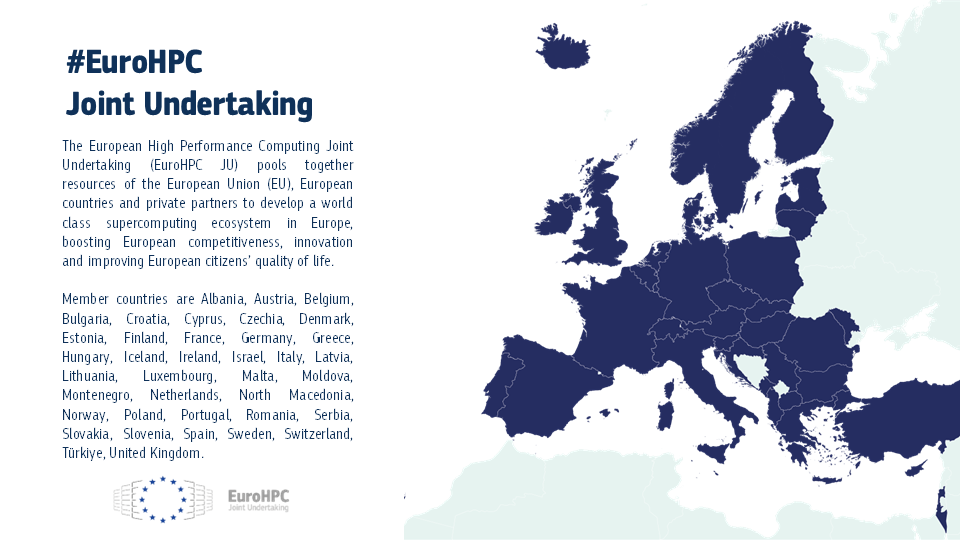
\includegraphics[width=0.72\textwidth]{graphics/eurohpc-participating-states.png}
        {\scriptsize\textcolor{SlidemintMuted}{EuroHPC JU participating states: 27 EU Member States + 11 associated countries $\Rightarrow$ 38.}}
    \end{center}

    \textcolor{SlidemintMuted}{There is no privileged access: EU projects line up through the same calls as everyone else.}
\end{frame}

\begin{frame}
    \frametitle{The application workflow}
    \framesubtitle{From call to first job}
    \begin{enumerate}
        \item \SlidemintTextbf{Choose the access mode.} Six modes with very different latencies (see \emph{Access modes that matter} and \emph{Access mode latency}).
        \item \SlidemintTextbf{Prepare the application.} The two hard fields for ML are scalability evidence and resource justification (see \emph{The application form} and \emph{What an academic can actually get}).
        \item \SlidemintTextbf{Submit through the portal} before the cutoff --- Benchmark and Development are continuously open.
        \item \SlidemintTextbf{Peer review:} independent panels rank the proposals; the JU took this over from PRACE at the end of 2022.
        \item \SlidemintTextbf{Start computing} with the awarded allocation and host-site accounts.
    \end{enumerate}

    \vspace{2em}
    \textcolor{SlidemintMuted}{Throughput $\approx$ GPUs $\times$ reliability $\times$ queue $\times$ proposal latency $\times$ communication.}
\end{frame}

\begin{frame}
    \frametitle{Free of charge means having obligations}
    \framesubtitle{What successful applicants commit to}
    \begin{itemize}
        \item \SlidemintTextbf{Acknowledge} EuroHPC resources in all related publications.
        \item Contribute to \SlidemintTextbf{dissemination} events.
        \item Submit a \SlidemintTextbf{final report} after the allocation ends.
    \end{itemize}

    \vspace{1em}
    The exact conditions are set per call --- read the call's documents before applying.

    \vspace{2em}
    \textcolor{SlidemintMuted}{Free of charge $\neq$ free of effort.}
\end{frame}

\begin{frame}
    \frametitle{Where to get help along the way}
    \framesubtitle{Two support tiers}
    \SlidemintTextbf{EPICURE} (EuroHPC Application Support) provides \SlidemintEmph{Level 2/3} services:
    \begin{itemize}
        \item code enabling and \SlidemintTextbf{scaling} across EuroHPC systems
        \item \SlidemintTextbf{performance analysis} and benchmarking
        \item \SlidemintTextbf{code refactoring} and optimization
    \end{itemize}

    \vspace{0.8em}
    \SlidemintTextbf{Level 1} (accounts, logins, queues, basic job scripts) stays with the \SlidemintTextbf{host site's application support} team.

    \vspace{2em}
    \textcolor{SlidemintMuted}{Porting to a new architecture is real work --- budget time for it.}
\end{frame}

\section{MINERVA: the European AI support hub}

\begin{frame}
    \frametitle{MINERVA}
    \framesubtitle{The European Support Centre for Scalable AI Research and Deployment}
    A EuroHPC JU-funded project (2025--2027) that helps European AI research
    teams make real use of HPC: \SlidemintTextbf{free support} for porting,
    scaling, and training large models on EuroHPC systems.

    \vspace{0.8em}
    \begin{itemize}
        \item \SlidemintTextbf{Access to state-of-the-art HPC} infrastructure via EuroHPC JU calls.
        \item \SlidemintTextbf{Scaling and optimization} of AI workflows by HPC-AI specialists.
        \item \SlidemintTextbf{Training}, best practices, and a European community hub.
        \item Strengthens \SlidemintTextbf{open foundation models} and European digital sovereignty.
    \end{itemize}

    \vspace{1em}
    \textcolor{SlidemintMuted}{minerva4ai.eu}
\end{frame}

\begin{frame}
    \frametitle{MINERVA support tiers}
    \framesubtitle{Free help from ``port it'' to ``reach its full performance''}
    \begin{itemize}
        \item \SlidemintTextbf{L1} -- porting AI applications and workflows to HPC
        \item \SlidemintTextbf{L2} -- using and mastering AI libraries (PyTorch, TensorFlow) on HPC architectures
        \item \SlidemintTextbf{L3} -- pre-training open large-scale and foundation models
        \item \SlidemintTextbf{L4} -- specializing open large-scale and foundation models
        \item \SlidemintTextbf{L5} -- guidance on ethical and responsible AI
    \end{itemize}

    \vspace{1em}
    \textcolor{SlidemintMuted}{Funded by the European Union / EuroHPC JU; coordinated by CINECA with BSC, J\"ulich, CEA/CNRS/CINES, and more.}
\end{frame}

\begin{frame}
    \frametitle{MINERVA's grant tools}
    \framesubtitle{Two free assistants, from application to request}
    \begin{description}
        \item[\SlidemintTextbf{HPC Grant Studio} (\texttt{hpcgrants.minerva4ai.eu})]
        your \SlidemintTextbf{hub for free GPU compute} in Europe: pick the right
        EuroHPC call (AI Factory, Benchmark, Development Access, \dots), step
        through the application, and check your fit -- directly on the MINERVA
        portal.
        \item[\SlidemintTextbf{Compute Needs Estimator} (\texttt{estimator.minerva4ai.eu})]
        turn a research plan into a \SlidemintTextbf{credible GPU-hour request}:
        workload, model family, data, precision, GPUs $\to$ an estimate with
        \SlidemintTextbf{transparent methodology} and a justification you can reuse.
    \end{description}

    \vspace{1em}
    \textcolor{SlidemintMuted}{Both are free, developed within MINERVA, and point you to the right access call.}
\end{frame}

\begin{frame}
    \frametitle{The Compute Needs Estimator}
    \framesubtitle{From ``I want to train a model'' to a justified allocation}
    \begin{itemize}
        \item \SlidemintTextbf{Workload}: full-model training, partial fine-tuning, PEFT/LoRA, or inference/evaluation.
        \item \SlidemintTextbf{Experimentation}: one-shot, regular iteration, heavy R\&D, or paper-ready ablations.
        \item \SlidemintTextbf{Model size} and \SlidemintTextbf{data}: parameter count, dataset volume, epochs.
        \item \SlidemintTextbf{Efficiency}: compute precision, target GPU count (up to 128).
    \end{itemize}

    \vspace{0.6em}
    Output: \SlidemintTextbf{GPU-hours by architecture} (V100 / A100 / H100),
    estimated wall-clock time, \SlidemintTextbf{VRAM / node} analysis, and a
    \SlidemintTextbf{request recommendation} (GPU type, access call, copy-able
    justification for the application).

    \vspace{1em}
    \textcolor{SlidemintMuted}{Estimator is advisory and methodology-based; used e.g.\ to size a Jean Zay request.}
\end{frame}

\begin{frame}
    \frametitle{MINERVA Best Practice Guides}
    \framesubtitle{Optimizing AI models on European infrastructure}
    A free, open guidebook that bridges \SlidemintTextbf{AI practice and HPC practice} --
    the ``why'' behind systems behavior plus recipes for shared supercomputers.

    \vspace{0.8em}
    \begin{itemize}
        \item \SlidemintTextbf{1. Infrastructure Foundations} -- compute, GPU architectures, networking, storage, scheduling.
        \item \SlidemintTextbf{2. Efficient and Reliable LLM Pretraining} -- parallelism, scaling, sustainability, checkpointing, evaluation.
        \item \SlidemintTextbf{3. Post-Training} -- instruction tuning, alignment (RL), efficient inference.
        \item \SlidemintTextbf{4. Explainable AI} -- interpretability methods with Jupyter notebooks and use cases.
    \end{itemize}

    \vspace{0.8em}
    \textcolor{SlidemintMuted}{best-practice-guides.minerva4ai.eu\ \,\textbar\, CC~BY~4.0 (text), Apache~2.0 (code).}
\end{frame}

\section{How to use HPC}

\begin{frame}
    \frametitle{Let's make use of what we've been given!}
    An experiment workflow that survives
    \begin{itemize}
        \item queues
        \item failures and maintenance
        \item fairshare
        \item filesystem weirdness
        \item conference deadlines
    \end{itemize}
\end{frame}

\begin{frame}[fragile]
    \frametitle{1. Keep one local source of truth}
    \framesubtitle{Code and data}
    \begin{columns}[t]
        \begin{column}{0.50\textwidth}
        \begin{minted}{text}
            project/
              pyproject.toml
              uv.lock
              src/
              scripts/
              configs/
              data_manifest.toml
              experiments/
                2026-05-19_param_grid/
              results/
                metrics.jsonl
        \end{minted}
        \end{column}

        \begin{column}{0.48\textwidth}
        The cluster is a \SlidemintTextbf{worker}.

        \vspace{0.5em}
        Code $\to$ git + \mintinline{bash}|rsync|

        \vspace{0.5em}
        Data $\to$ explicit snapshots, backed up locally.

        \vspace{3em}
        When \mintinline{bash}|$WORK| is in emergency maintenance and your only experiment config lives there, you are very stressed. Ask me how I know.
        \end{column}
    \end{columns}
\end{frame}

\begin{frame}[fragile]
    \frametitle{2. Submit many small jobs}
    Small jobs:
    \begin{enumerate}
        \item fit into scheduler holes;
        \item fail cheaply;
        \item give partial information earlier.
    \end{enumerate}

    \vspace{2em}
    \textcolor{SlidemintMuted}{``Small'' here means \SlidemintTextbf{restartable + interpretable}: one seed, one shard, one attack config.}
\end{frame}

\begin{frame}[fragile]
    \frametitle{3. Make long jobs resumable}

    \begin{itemize}
        \item Ask for 3--12 hours, repeatedly, instead of 3 days at once.
        \item A useful checkpoint contains \SlidemintEmph{more than weights}:
            \begin{minted}{python}
                checkpoint_keys = {
                    "step", "model", "optimizer", "scaler", "torch_rng",
                    "numpy_rng", "python_rng", "config_hash", "git_commit",
                }
            \end{minted}
        \item Write atomically:
            \begin{minted}{python}
                tmp = path.with_suffix(".tmp")
                torch.save(state, tmp)
                os.replace(tmp, path)
            \end{minted}
        \item On SLURM, ask for a warning and checkpoint inside Python:
            \begin{minted}{bash}
                #SBATCH --signal=B:USR1@120
            \end{minted}
    \end{itemize}

    \vspace{0.1em}
    \textcolor{SlidemintMuted}{Bonus: with resumability, \SlidemintTextbf{preemptable nodes} cost you nothing.}
\end{frame}

\begin{frame}[fragile]
    \frametitle{4. Encode dependencies}
    \framesubtitle{\mintinline{bash}|sbatch| is a DAG submitter}
    SLURM dependencies: \mintinline{text}|afterok|, \mintinline{text}|afterany|, \mintinline{text}|afternotok|, \mintinline{text}|aftercorr|, \mintinline{text}|singleton|.

    \vspace{0.4em}
    \begin{minted}[fontsize=\scriptsize]{bash}
        PRE=$(sbatch --parsable preprocess.sh)
        TRAIN=$(sbatch --parsable --dependency=afterok:$PRE --array=0-63%8 train.sh)
        EVAL=$(sbatch --parsable --dependency=aftercorr:$TRAIN --array=0-63%16 eval.sh)
        sbatch --dependency=afterok:$EVAL aggregate.sh
    \end{minted}

    \vspace{0.4em}
    On HTCondor: \SlidemintTextbf{DAGMan}.

    \vspace{2em}
    \textcolor{SlidemintMuted}{Cleaner than polling \mintinline{bash}|squeue| every five minutes.}
\end{frame}

\begin{frame}
    \frametitle{5. Optimize the code}
    For LLM work, benchmark:
    \begin{itemize}
        \item attention: eager / SDPA / FlashAttention
        \item bf16 / fp16 / fp32
        \item gradient checkpointing on/off
        \item batch size, sequence length, dataloader workers, pinned memory
    \end{itemize}

    \vspace{1em}
    Small plug: \href{https://github.com/bmucsanyi/autobatch}{autobatch} for ``what batch size fits?''

    \vspace{1em}
    Slow code is \SlidemintTextbf{communal financial damage} and large-scale grants require code reviews beforehand.
\end{frame}

\begin{frame}[fragile]
    \frametitle{Source of truth for results, too}
    Every result should know:
    \vspace{1em}

    \begin{minted}[fontsize=\scriptsize]{python}
result_fields = [
    "run_id", "cluster", "job_id", "git_commit", "config_hash",
    "data_revision", "model_revision", "seed", "gpu_type", "num_gpus",
    "started_at", "ended_at", "wallclock_hours", "gpu_hours", "status",
]
    \end{minted}

    \vspace{0.4em}
    ``The same experiment across Ferranti, Helix, MN5, and whatever was up this week.''
\end{frame}

\begin{frame}[fragile]
    \frametitle{A few commands to actually use}
    \begin{columns}[t]
        \begin{column}{0.49\textwidth}
        \SlidemintTextbf{SLURM}
        \begin{minted}{bash}
            squeue --me
            squeue --me --start
            scontrol show job <JOBID>
            sacct -j <JOBID> --format=...
            seff <JOBID>
            sshare -u $USER
            scancel <JOBID>
            scancel --state=PENDING
        \end{minted}
        \end{column}

        \begin{column}{0.49\textwidth}
        \SlidemintTextbf{HTCondor}
        \begin{minted}{bash}
            condor_q $USER
            condor_q -run $USER
            condor_rm <ClusterId>
            condor_ssh_to_job <Id.Proc>
            condor_submit_bid 50 job.sub
            condor_change_bid 100 <Id>
        \end{minted}
        \end{column}
    \end{columns}

    \vspace{0.6em}
    \SlidemintTextbf{The most underrated:} the one that tells you what you actually used.
\end{frame}

\section{Closing}

\begin{frame}[fragile]
    \frametitle{Three takeaways}
    \begin{enumerate}
        \item \SlidemintTextbf{Throughput} $\approx$ GPUs $\times$ reliability $\times$ queue $\times$ proposal latency $\times$ communication.\\
              The cluster's \mintinline{bash}|sinfo| is the smallest factor of that product.
        \item \SlidemintTextbf{Climb the ladder:} desktop $\to$ university $\to$ state $\to$ federal \SlidemintTextbf{(NHR, GCS)} $\to$ EuroHPC.
        \item \SlidemintTextbf{Workflow:} Small jobs, resumability, DAGs, one local source of truth, efficient code.
    \end{enumerate}

    \vspace{2em}
    \textcolor{SlidemintMuted}{Free of charge $\neq$ free of effort; proposal time and setup time is real time.}
\end{frame}

\begin{frame}
    \frametitle{Questions?}
    \begin{center}
        \textcolor{SlidemintMuted}{\small Michael Tiemann}

        \vspace{2.5em}

        
\includegraphics[height=1.1cm]{graphics/minerva-logo.png}
        \hspace{2em}
        
\includegraphics[height=1.1cm]{graphics/eu-cofunded.jpg}
    \end{center}
\end{frame}

\begin{frame}[allowframebreaks]
    \frametitle{References}
    \bibliographystyle{plainnat}
    \bibliography{references}
\end{frame}

\end{document}
